\documentclass[../main.tex]{subfiles}
\graphicspath{{\subfix{../images/}}}
\begin{document}


\begin{figure}[htb!]
\centering
  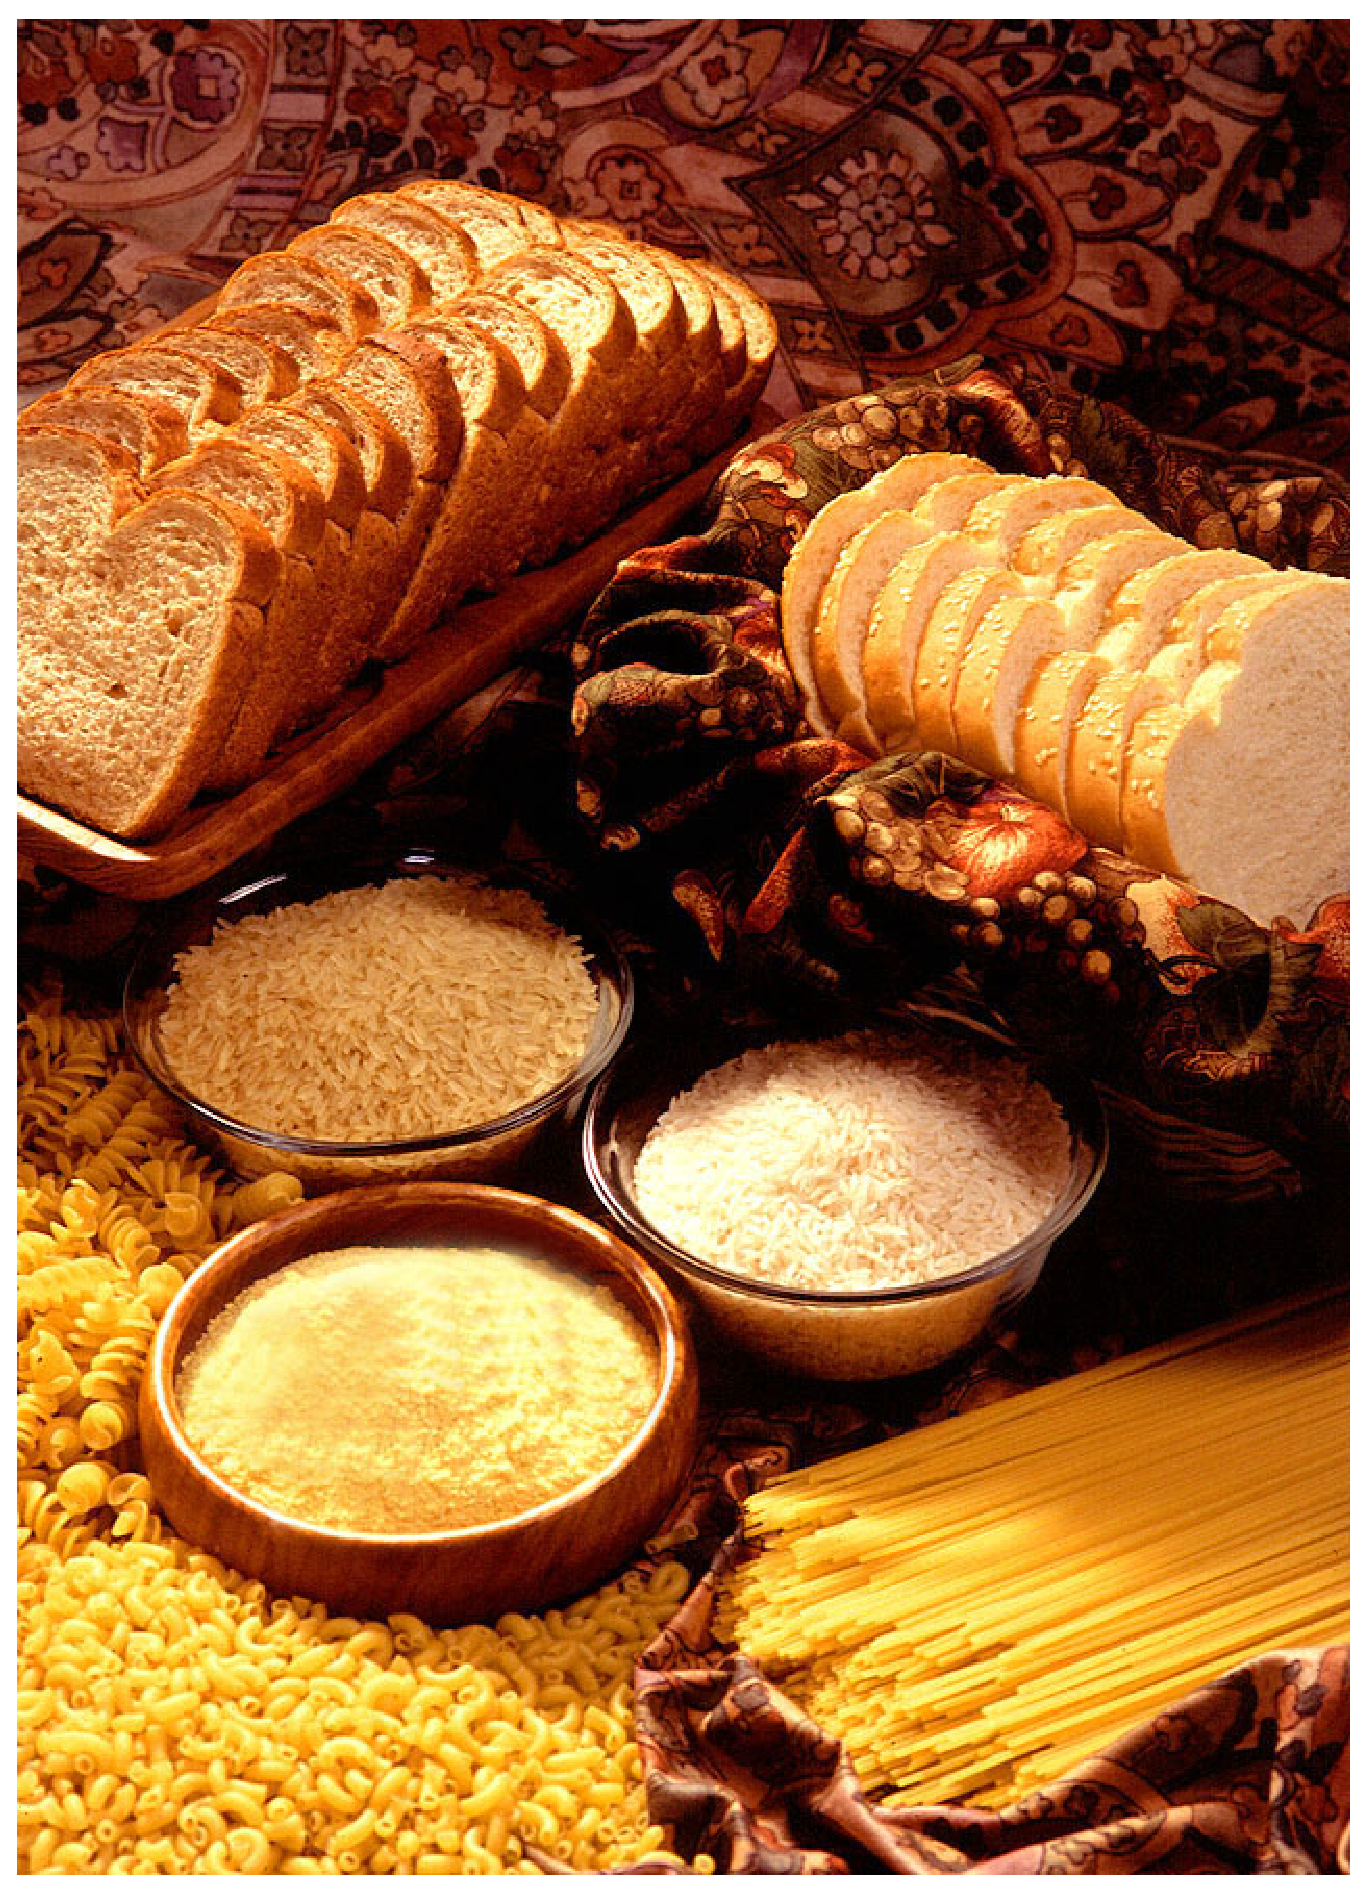
\includegraphics[width=7cm]{starchy-foods}
  \caption{Foods rich in carbohydrates~\cite{PicCarbohydrates}}
\end{figure}


Carbohydrates\index{carbohydrate} (also called saccharides) are the most important sources of fuels for the human body, by amount.
Especially the brain is highly dependent on carbohydrates as fuel sources, given that it can't combust fats, contrary to muscles.
One gram of carbohydrates provides 4 kcal (17 kJ) of energy, one ounce 113 kcal or 482 kJ.
The human body can build all carbohydrates from proteins and glycerol, a constituent of fat, so therefore are carbohydrates not essential.
Nevertheless should the sufficient supply of carbohydrates be part of the daily food intake.
Else there's a risk that valuable proteins of the body are depleted (for instance muscles).
An excess of carbohydrates can be stored on a short term base in the liver (\sfrac{1}{3}) and in the muscle tissue (\sfrac{2}{3}) in the form of glycogen.
The carbohydrate storage capacity is very small, as opposed to the fat storage capacity, which is almost limitless.
These carbohydrate reserves are getting tapped into when a fast straining performance is required, for instance flight from an enemy.
In an untrained person, they are enough for about 45 minutes of endurance running.
If our body gets more carbohydrates than necessary for maintaining the energy, the excess gets transformed into fats and stored in the form of body fats.

Carbohydrates (or saccharides) have the following characteristics:
\begin{itemize}
\item important source of energy for the cells
\item being able to be stored in liver and muscles in the form of glycogen\index{glycogen}\index{storage!sugar} on a short term base
\item maintaining the body temperature
\end{itemize}

\subsection{Structure of Carbohydrates}

The term carbohydrates\index{carbohydrate} comes from the chemical composition of this food constituent.
They are \emph{carbon} chains which are connected to water molecules, $H_2O$, (\emph{hydrate}d).
Carbohydrates can be separated onto the following categories:
\begin{description}
\item[digestible carbohydrates] like sugar and starch
\item[non--digestible carbohydrates] like fibers\index{fiber} (see chapter fibers, chapter~\ref{chap:fibers}, p.~\pageref{chap:fibers})
\end{description}

The carbohydrates are composed from the basic building blocks, the saccharides (sugar).
We distinguish monosaccharides, disaccharides, oligosaccharides and polysaccharides, with one, two, multiple or many sugar units respectively.

\subsection{Fast and Slow Carbohydrates}

\subfile{TableSugar.tex}

Monosaccharides are ``fast sugars'' (eg. sweet drinks, white flour, sweets, \ldots).
They can get absorbed directly by the body without further processing in the colon, even already through in mucous membranes of the mouth.
They cause a fast increase in blood sugar levels, they spike them.

Disaccharides and polysaccharides are ``slow sugars'' (eg. whole grain bread, potatoes, grains,\ldots).
They consist of multiple monosaccharide units linked up into a chain.
Before being digested, they have to be cleaved into glucose\index{glucose},
a monosaccharide unit, in order to be able to be passed into to the blood.
Such slow sugars increase the blood sugar level only slowly and continuously.

Foods, which contain slow sugars should be preferred for our consumption.
Further details see chapter glycemic index/glycemic load, chapter~\ref{glycemic}, p.~\pageref{glycemic}.



\begin{table}[htb]
  \centering
  \begin{tabular}{p{\textwidth}}
    \textbf{Carbohydrate intake (daily)} \\
    Reference values in \% of the daily caloric intake (reference values DACH 2000) \\
    \hline
    Around 50\% carbohydrates \\
    \tabitem preferably in the form of starch \\
    \tabitem carefully dealing with added types of sugars*\\
    \footnotesize{*according to the WHO, the amount of added sugars and sweeteners (ie. honey)  should be a maximum of 10\% of the daily caloric intake} \\
    \vspace{5mm}
    A carbohydrate amount of 50\% corresponds to: \\
    \hline
    2000 kcal: 250 g. (8\sfrac{3}{4} oz) of carbohydrates and max. 50 g (1\sfrac{3}{4} oz) sugars/sweeteners\\
    3000 kcal: 375 g. (13\sfrac{1}{4} oz) of carbohydrates and max. 75 g (2\sfrac{1}{2} oz) sugars/sweeteners\\
    
  \end{tabular}
  \caption[Carbohydrate daily needs]{How many carbohydrates does a human being need?}
\end{table}


 
\vspace{5mm}
\noindent
\begin{fminipage}{\textwidth}
  \textbf{Profile Carbohydrates}
  \begin{itemize}
  \item carbohydrates = Saccharides
  \item 1 g (\sfrac{1}{8} oz) deliver 4 kcal or 17 kJ (14\sfrac{1}{8} kcal or 60\sfrac{1}{4} kJ) of energy
  \item classification: Mono-- (simple), Di-- (double) and polysaccharides (multiple sugar units)
  \item carbohydrate intake: 50\% of the daily intake and thereof max. 10\% monosaccharides
  \item carbohydrates out of foods rich in starch and fibers are also rich in vitamins, minerals and secondary plant nutrients (phytonutrients)
    \item fibers = indigestible carbohydrates
  \end{itemize}
\end{fminipage}


\end{document}